% \section{Motivation}
% \label{sec:motivation}

% % Does adding a threat model section make sense?
% \amirian{Given the intro, I think we can safely remove this section. I've tried to work in pertinent parts into the intro}

% % but whatever works for lambdas is applicable to containers & VMs...
% % can we definitively say this?

\section{Methodology}
\label{sec:methodology}

% TODO: This figure shows only mem access latencies of exotic 
% operation. how does these operations affect latencies of other exotic 
% operations or regular memory accesses?
\begin{figure*}[h!]
\begin{subfigure}{.33\textwidth}
  \centering
  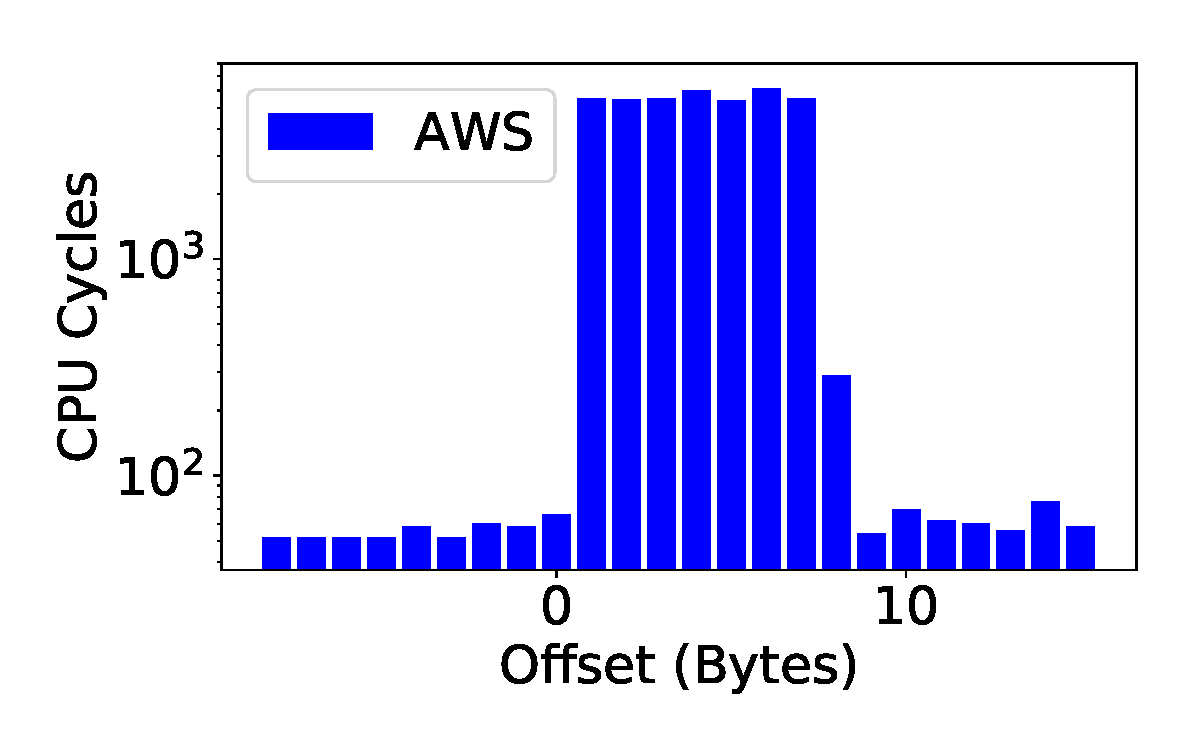
\includegraphics[width=.99\linewidth]{fig/membus_aws.pdf}
%   \caption{1a}
%   \label{fig:sfig1}
\end{subfigure}%
\begin{subfigure}{.33\textwidth}
  \centering
  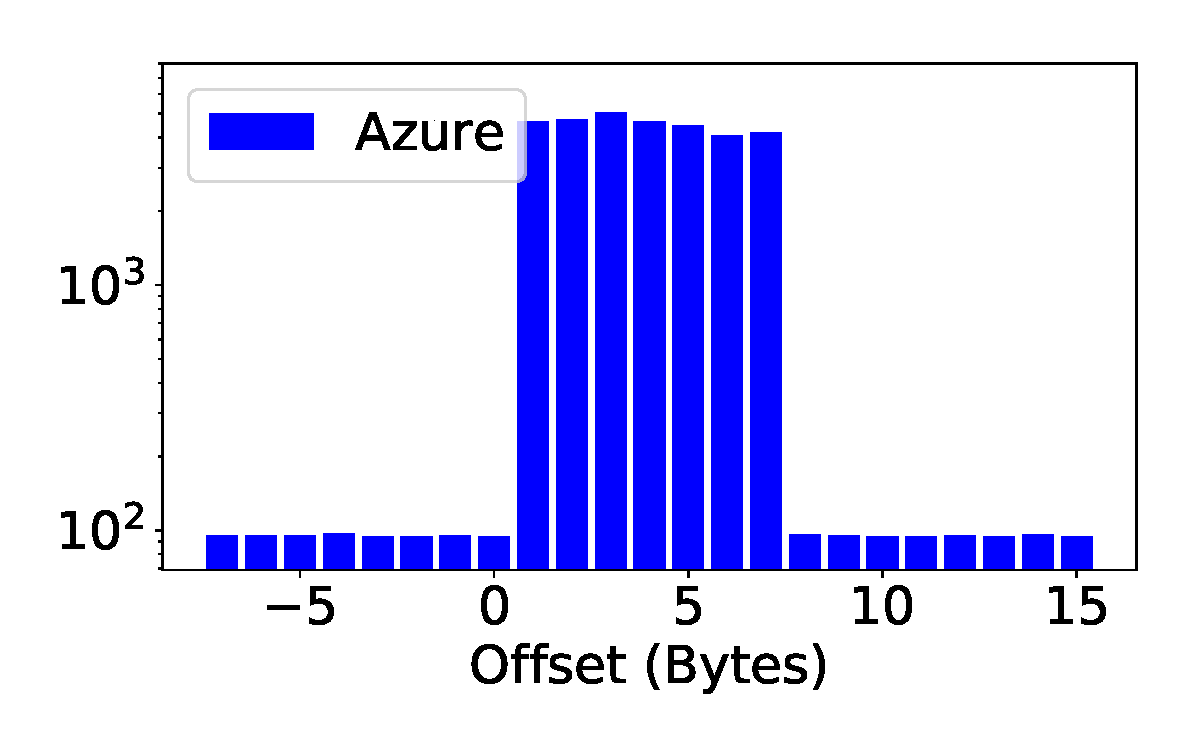
\includegraphics[width=.99\linewidth]{fig/membus_azure.pdf}
%   \caption{1b}
%   \label{fig:sfig2}
\end{subfigure}
\begin{subfigure}{.33\textwidth}
  \centering
  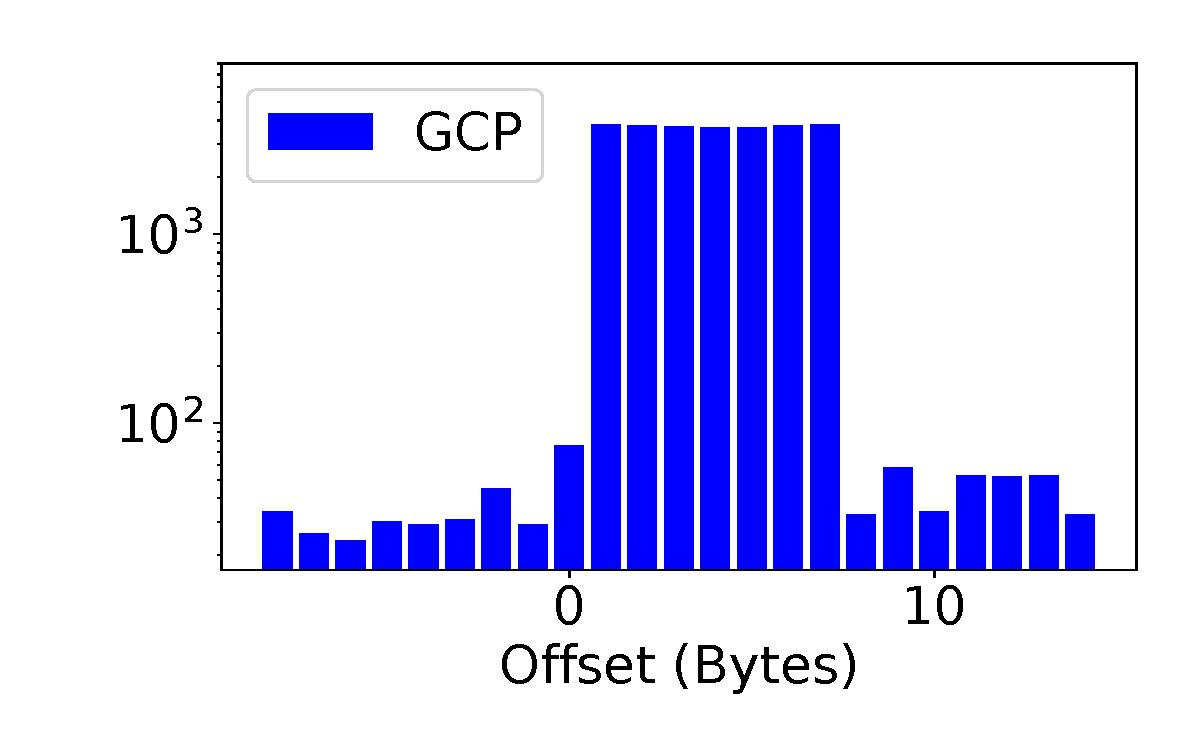
\includegraphics[width=.99\linewidth]{fig/membus_gcp.pdf}
%   \caption{1b}
%   \label{fig:sfig2}
\end{subfigure}
\caption{The plots show the latencies of atomic memory operations performed on
        an 8B memory region as we slide from one cache line across the boundary into
        another on AWS, Azure, and Google (GCP) respectively.  The latencies are orders
        of magnitude higher when the 8B region falls across the two cache lines (offsets
        0-7B), demonstrating the presence of the memory bus covert channel on all these
        cloud providers. \label{fig:membus_clouds}}
\label{fig:fig}
\end{figure*}


Our goal is to determine a (co-operative) co-residence detection mechanism for
lambdas. In other words, given a series of spawned lambdas in a
certain region of a cloud service, how can we determine the lambdas that are
co-resident on the same machines?  In this section, we discuss the details of
such a mechanism, previous solutions to this problem, and the unique challenges
we faced with lambda co-residence.

Given a set of cloud instances (VMs, Containers, Functions, etc) deployed to a
public cloud, a co-residence detection mechanism should identify, for each pair
of instances in the set, whether the pair was running on the same physical
server at some point. Paraphrasing Varadarajan et al.~\cite{varadarajan2015},
for any such mechanism to be useful across a wide range of launch strategies, it
should have the following properties:

\begin{itemize}
    \item \textbf{Generic} The technique should be applicable across a wide
    range of server architectures and software runtimes. In practice, the
    technique would work across most third-party cloud platforms and even among different
    platforms within a cloud.
    \item \textbf{Reliable} The technique should have a reasonable detection success
    with minimal false negatives (co-resident instances not detected) and even 
    less false positives (non co-resident instances categorized as co-resident).
    \item \textbf{Scalable} A launch strategy may require hundreds or even
    thousands of instances to be deployed, and must scale such that the
    technique will detect all co-resident pairs at a reasonable cost.
\end{itemize}

\noindent We add another property to that list which is relevant to lambdas:
\begin{itemize}
    \item \textbf{Fast} The technique should be fast, preferably finishing in 
    the order of seconds. As lambdas are ephemeral (with some clouds restricting their 
    execution times to as low as a minute), the technique should leave ample time 
    for other activities that make use of the resulting co-resident information.
\end{itemize}

Given these properties, we decide to investigate harware-based covert channels.
Hardware-based covert-channels are more difficult to remove and obfuscate than
software-based covert channels, and are more pervasive, 
given that hardware is more homogenous across computing platforms than software. 

\subsubsection{Memory bus channel}
We utilize the memory bus covert channel described in
section~\ref{sec:background:covertchannels} as it exploits a fundamental
hardware vulnerability that is present across all generations of x86 hardware.
Historically, multiple public cloud services have been vulnerable to this
channel~\cite{varad191016,zhang2016}, and we ffind that they are still
vulnerable today. To demonstrate the presence of the vulnerability, we measure
the latency of atomic operations on a 8B memory region as we slide the region
from one cacheline into another across the cacheline boundary. We perform this
experiment on three major cloud platforms (AWS, Google and Microsoft Azure) and
show the latencies observed in Figure~\ref{fig:membus_clouds}. From the figure,
we can see that all three cloud platforms still exhibit a significant difference
in latencies for the "exotic" memory locking operations (where the memory region
falls across cacheline boundary) when compared to regular memory accesses,
demonstrating the presence of this covert channel on all of them. Moreover, we
were able to execute these experiments on serverless function instances. Since
lambdas have runtimes that are generally restricted to high-level languages
(that prevent the pointer arithmetic required to perform these exotic
operations), we used the unsafe environments on these clouds --- C++ on AWS,
Unsafe Go on GCP, Unsafe C\# On Azure. This shows the applicability of using the
covert channel across different kinds of cloud instances as well.


% why previous approaches were not scalable
\subsubsection{Previous approaches}
Previous works that used the memory bus for co-residence detection divide the
deployed instances into sender and receiver roles, and attempt to identify the
sender role with a receiver role. The sender instances continually lock the
memory bus (locking process) for a certain duration (\textasciitilde 10 seconds)
while the receiver samples the memory for any spike in access latencies (probing
process). If all the deployed instances try the detection i.e., locking and
probing at once, (some of) the receivers may see locking effects, but there
would be no way of knowing which or how many senders are co-resident with a
particular receiver and caused the locking. This provides no information about
the number of physical servers that ran these instances or the amount of
co-residence. The only information we can deduce is that receivers were probably
co-resident with at least a single sender.

An alternative method is to try pair-wise detection where one sender instance
locks and one receiver instance probes at a time, revealing co-residence of this
pair, and repeating this serially for each pair. However, this technique is too
slow and scales quadratically with the number of instances e.g., a hundred
instances would take more than 10 hours assuming 10 secs for each pair.
Varadarajan et al.~\cite{varad191016} speed up this process significantly by
performing detection for mutually-exclusive subsets in parallel, allowing for
false-positives and later eliminating the false-positives sequentially. This
would only scale linearly in the best case, which is still expensive; with a
thousand instances, for example, the whole detection process takes well over two
hours to finish, which is infeasible for lambdas that are, by nature, ephemeral.
Thus, one challenge in this work is creating a faster co-residence
algorithm.

% how do we scale it - challenges.
\subsubsection{The Path to Scalability}

%One challenge in creating a lambda neighbor detection algorithm is speed. - repeated
One method to quicken the co-residence process is by decreasing the time a single
sender-receiver pair requires to determine co-residence (i.e., improving upon
probing time and accuracy of the receiver). However, this method only affects
total time by a constant factor. To improve scalability, we need to
run the detection for different sender-receiver pairs in parallel without
sacrificing the certainty of information we receive when they are run serially.  For
example, when two pairs observe co-residence, we must be certain that each
receiver experienced co-residence because of its own paired sender instance, which
is not possible if co-residence is ascertained based a simple yes/no signal from
the sender instances. 

Given that previous work utilized the memory bus channel to exchange more
complex information like keys~\cite{wuusenix2012}, it appears that the memory
bus can be used to exchange information, such as unique IDs, between the
co-resident instances, allowing us to ascertain receiver/sender pairs.  However,
the previous work assumes that there is only one sender and one receiver that
know exactly how and when to communicate. As we will see in the next section,
this model is not sustainable when there exist many parties that have no
knowledge of each other but try to communicate on the same channel.

To solve some of the challenges mentioned previously, we propose a protocol in
which we use the memory bus covert channel to exchange information between the
instances that have access to the channel. Using the protocol, co-resident
instances can reliably exchange their unique IDs with each other to discover
their neighbors. The protocol takes time on the order of number of instances
involved, which is limited by the maximum number of co-located instances on a
single server (tens), a number that is orders of magnitude less than the total
number of instances deployed to the cloud (hundreds to thousands). Removing this
dependency on total number of instances deployed allows us scale our co-residence
detection significantly, as we will see the the next section.
